\section{Boussinesq}
\label{sec:boussinesq}

In this section, we present the results of our analysis, beginning with the simplest
stratification model, namely the Boussinesq limit. Given the novelty of the framework and its
stochastic character, we first validate the formulation by comparing the predicted mean energy
growth with ensembles of three-dimensional direct numerical simulations.

For this comparison, we use the \(n=1\) spectrum defined in~\eqref{eq:eta_spectrum_family} and
compare against the triperiodic pseudo-spectral solver
PsDNS\footnote{\url{https://github.com/lanl/PsDNS.git}}, developed at LANL and designed to solve
the incompressible Navier--Stokes equations with buoyant forcing. This model corresponds to the
limit \(\Atw \to 0\) of the present formulation~\citep{livescu-ristorcelli-2007}. The results are
reported in figure~\ref{fig:compare_dns}, showing good agreement between the mean energy growth
predicted by the stochastic theory and the ensemble mean extracted from ten independent numerical
simulations, across several values of the horizontal correlation length \(\lambda\).

\begin{figure}
    \centering
    % This file was created by matlab2tikz.
%
\definecolor{mycolor1}{rgb}{0.91400,0.56100,0.47800}%
\definecolor{mycolor2}{rgb}{0.83900,0.37600,0.30200}%
\definecolor{mycolor3}{rgb}{0.64700,0.12900,0.14500}%
\definecolor{mycolor4}{rgb}{0.40400,0.00000,0.12200}%
%
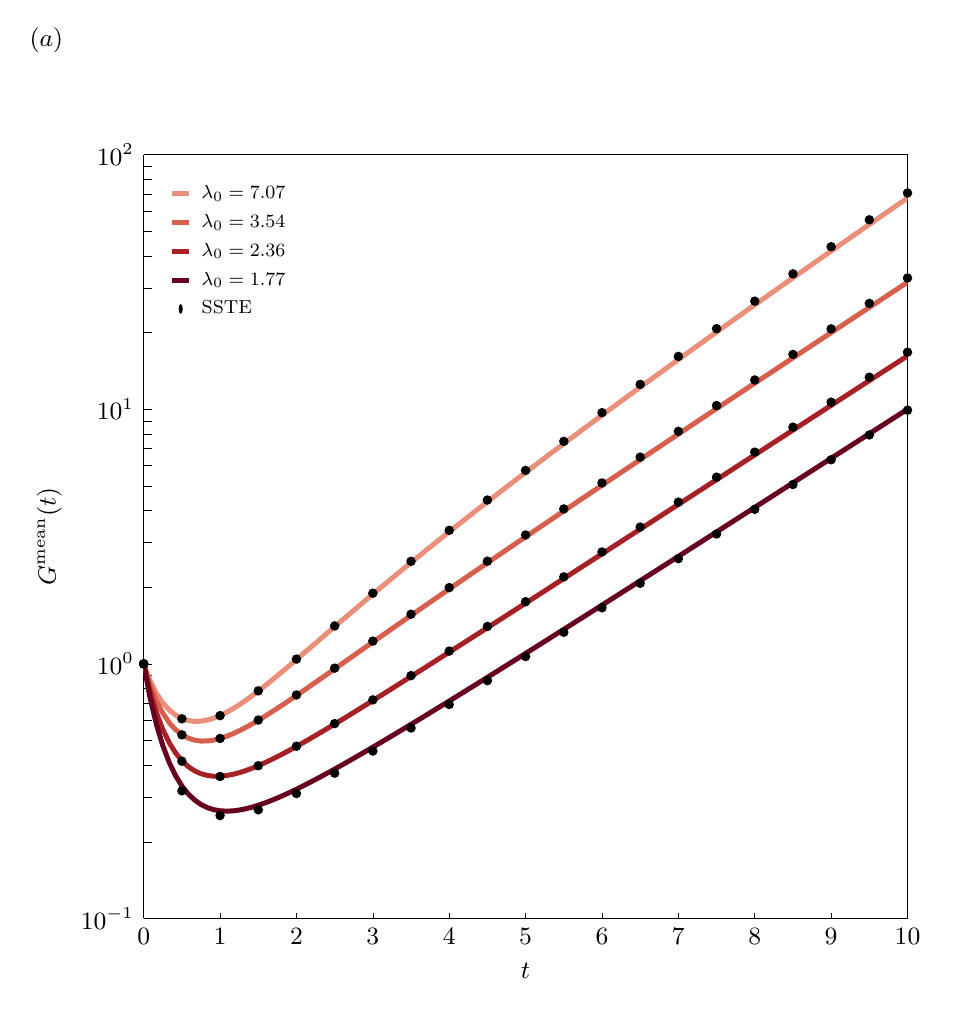
\begin{tikzpicture}

\begin{axis}[%
width=11.252in,
height=7.131in,
at={(1.887in,0.962in)},
scale only axis,
clip=true,
separate axis lines,
every outer x axis line/.append style={black},
every x tick label/.append style={font=\color{black}},
every x tick/.append style={black},
xmin=0,
xmax=10,
xlabel={$t$},
every outer y axis line/.append style={black},
every y tick label/.append style={font=\color{black}},
every y tick/.append style={black},
ymode=log,
ymin=0.1,
ymax=100,
yminorticks=true,
ylabel={$\mathscr{G}^{\mathrm{mean}}(t)$},
axis background/.style={fill=white},
legend style={at={(0.03,0.97)}, anchor=north west, legend cell align=left, align=left},
clip=true,
clip mode=individual,
axis lines=box,
xtick pos=bottom,
ytick pos=left,
tick align=inside,
major tick length=2pt,
width=0.8\linewidth,
height=0.8\linewidth,
every axis/.append style={font=\fontsize{9}{9}\selectfont},xlabel style={font=\fontsize{9}{9}\selectfont},title style={font=\fontsize{9}{9}\selectfont},
legend style={font=\fontsize{8}{9}\selectfont,inner sep=1pt,row sep=1pt,column sep=2pt,nodes={scale=0.85},draw=none},legend image post style={xscale=0.35},
legend columns=1,
scaled x ticks=false,
tick label style={/pgf/number format/fixed,/pgf/number format/precision=2},
every x tick label/.append style={font=\fontsize{9}{9}\selectfont\color{black}},
every y tick label/.append style={font=\fontsize{9}{9}\selectfont\color{black}},
,,
colormap={sigmamap}{rgb(0.0000)=(0.0200,0.1880,0.3800); rgb(0.1000)=(0.0743,0.3456,0.5616); rgb(0.2000)=(0.1918,0.4980,0.7060); rgb(0.3000)=(0.3890,0.6708,0.8226); rgb(0.4000)=(0.7552,0.8682,0.9228); rgb(0.5000)=(0.9690,0.9689,0.9689); rgb(0.6000)=(0.9425,0.8044,0.7614); rgb(0.7000)=(0.8767,0.4910,0.4020); rgb(0.8000)=(0.7869,0.2866,0.2470); rgb(0.9000)=(0.6186,0.1239,0.1568); rgb(1.0000)=(0.4040,0.0000,0.1220)}
]
\addplot [color=mycolor1, line width=1.8pt]
  table[row sep=crcr]{%
0	1\\
0.08	0.863137158521505\\
0.168	0.765296195121739\\
0.248	0.70474397683936\\
0.336	0.658588067607769\\
0.416	0.629965624874714\\
0.504	0.609519584109834\\
0.584	0.598892908179321\\
0.672	0.594352800620287\\
0.752000000000001	0.595723893901938\\
0.840000000000001	0.602453019766551\\
0.920000000000001	0.612775592295249\\
1	0.626711973705201\\
1.088	0.645872140261718\\
1.168	0.666532028500899\\
1.256	0.692615375910713\\
1.336	0.719241218543471\\
1.424	0.75161809759949\\
1.504	0.783785847991089\\
1.592	0.822122085993051\\
1.672	0.859627742041189\\
1.752	0.899650303696986\\
1.84	0.94658590309429\\
1.92	0.991917281242138\\
2.008	1.04474302259802\\
2.088	1.09549773591915\\
2.176	1.15438823944275\\
2.256	1.21076558561448\\
2.344	1.27598138132431\\
2.424	1.33825346035854\\
2.512	1.41013060368432\\
2.592	1.47863494697464\\
2.672	1.55024351361084\\
2.76	1.63271408325125\\
2.84	1.71116430192978\\
2.928	1.80141989337375\\
3.008	1.88719744834199\\
3.096	1.98580457936394\\
3.176	2.07945400275672\\
3.264	2.18704447946353\\
3.344	2.28917040355475\\
3.432	2.40644321391367\\
3.512	2.51771252197615\\
3.592	2.6335889910158\\
3.68	2.76658138177793\\
3.76	2.89270580804419\\
3.848	3.03742035263772\\
3.928	3.1746277528457\\
4.016	3.33202369135629\\
4.096	3.48122430690785\\
4.184	3.65234635855449\\
4.264	3.81453076764412\\
4.344	3.98327082575806\\
4.432	4.17675989630082\\
4.512	4.36010508177377\\
4.6	4.57031481138781\\
4.68	4.76948043259263\\
4.768	4.99780315637551\\
4.848	5.21410727490269\\
4.936	5.46205258737654\\
5.016	5.69692387401654\\
5.104	5.96612764098106\\
5.184	6.22111391381719\\
5.264	6.48625964894577\\
5.352	6.79012553863693\\
5.432	7.07790869573738\\
5.52	7.40769197688594\\
5.6	7.71999688768499\\
5.688	8.07785384695352\\
5.768	8.41671957503659\\
5.856	8.80498325633162\\
5.936	9.17261573798088\\
6.024	9.59380981525452\\
6.104	9.99259495760747\\
6.184	10.407109026888\\
6.272	10.8819664995123\\
6.352	11.3315143903061\\
6.44	11.8464706574774\\
6.52	12.3339470364914\\
6.608	12.8923125156637\\
6.68800000000001	13.4208459890154\\
6.77600000000001	14.0261982991293\\
6.85600000000001	14.5991696840653\\
6.93600000000001	15.1945683338136\\
7.02400000000001	15.876436477224\\
7.10400000000001	16.5217667285783\\
7.19200000000001	17.2607682106632\\
7.27200000000001	17.9601231757078\\
7.36000000000001	18.7609370534059\\
7.44000000000001	19.5187369929625\\
7.52800000000001	20.3864158406654\\
7.60800000000001	21.207433434276\\
7.69600000000001	22.1474321520764\\
7.77600000000001	23.0368196368196\\
7.85600000000001	23.9606924910561\\
7.94400000000001	25.0183446871354\\
8.024	26.018949051088\\
8.11199999999999	27.1643640821777\\
8.19199999999998	28.2479219793519\\
8.27999999999997	29.4882088762784\\
8.35999999999997	30.6614326209336\\
8.44799999999996	32.0042598205101\\
8.52799999999995	33.2743891696673\\
8.61599999999994	34.7280268165682\\
8.69599999999993	36.1028687705243\\
8.77599999999992	37.5304930532827\\
8.86399999999991	39.1642054407962\\
8.9439999999999	40.7091946766412\\
9.03199999999989	42.4770841710685\\
9.11199999999988	44.1488397483288\\
9.19999999999987	46.0616415823677\\
9.27999999999986	47.870293520584\\
9.36799999999985	49.9395735308096\\
9.44799999999985	51.8960342800602\\
9.52799999999984	53.9269569894389\\
9.61599999999983	56.2502719535687\\
9.69599999999982	58.4466649750828\\
9.78399999999981	60.9590746898465\\
9.8639999999998	63.3340433754666\\
9.95199999999979	66.0505038538592\\
10.0319999999998	68.6181527059567\\
10.1199999999998	71.5547578800136\\
10.1999999999998	74.3302622980936\\
10.2879999999998	77.504325438466\\
10.3679999999997	80.5040080619984\\
10.4479999999997	83.6165323444928\\
10.5359999999997	87.17556024128\\
10.6159999999997	90.5386279632922\\
10.7039999999997	94.3838016223578\\
10.7839999999997	98.0169362234784\\
10.8719999999997	102.17051665725\\
10.9519999999997	106.09469307459\\
11.0399999999997	110.580591951725\\
11.1199999999997	114.818336213295\\
11.2079999999997	119.66222855866\\
11.2879999999996	124.237723147983\\
11.3679999999996	128.983059192458\\
11.4559999999996	134.406361683826\\
11.5359999999996	139.528410766155\\
11.6239999999996	145.381653212772\\
11.7039999999996	150.909191711203\\
11.7919999999996	157.225149158398\\
11.8719999999996	163.189023685422\\
11.9599999999996	170.002820882748\\
12.0399999999996	176.436081620031\\
12.1199999999996	183.105150249691\\
12.2079999999995	190.723383948328\\
12.2879999999995	197.914952576998\\
12.3759999999995	206.129096813346\\
12.4559999999995	213.882288496777\\
12.5439999999995	222.736852337883\\
12.6239999999995	231.093508923673\\
12.7119999999995	240.636080951151\\
12.7919999999995	249.640926243071\\
12.8799999999995	259.922357664499\\
12.9599999999995	269.623167158641\\
13.0399999999995	279.673109577726\\
13.1279999999994	291.14553911633\\
13.2079999999994	301.967923572421\\
13.2959999999994	314.320409887543\\
13.3759999999994	325.971339675488\\
13.4639999999994	339.267599744497\\
13.5439999999994	351.806868281739\\
13.6319999999994	366.114785496255\\
13.7119999999994	379.60607263263\\
13.7919999999994	393.574261837076\\
13.8799999999994	409.508988640465\\
13.9599999999993	424.530730198167\\
14.0479999999993	441.664553958808\\
14.1279999999993	457.814025783034\\
14.2159999999993	476.231044880986\\
14.2959999999993	493.587027276652\\
14.3839999999993	513.376519419052\\
14.4639999999993	532.02260770615\\
14.5519999999993	553.279264672947\\
14.6319999999993	573.304083115019\\
14.7119999999993	594.018101769329\\
14.7999999999993	617.62566226783\\
14.8799999999992	639.858881816661\\
14.9679999999992	665.192894843786\\
15.0479999999992	689.047311133611\\
15.1359999999992	716.223115297006\\
15.2159999999992	741.806489943681\\
15.3039999999992	770.94587927322\\
15.3839999999992	798.371943886715\\
15.4719999999992	829.603389177732\\
15.5519999999992	858.992043137176\\
15.6319999999992	889.359242283781\\
15.7199999999992	923.928405098054\\
15.7999999999991	956.446859195702\\
15.8879999999991	993.456276516502\\
15.9679999999991	1028.26195046884\\
16.0559999999991	1067.86489056044\\
16.1359999999991	1105.10052651647\\
16.2239999999991	1147.45779408721\\
16.3039999999991	1187.27305534548\\
16.3839999999991	1228.37135237476\\
16.4719999999991	1275.10473645266\\
16.5519999999991	1319.01650020257\\
16.6399999999991	1368.93573177344\\
16.719999999999	1415.82825788342\\
16.807999999999	1469.12134783689\\
16.887999999999	1519.16919198034\\
16.975999999999	1576.032162967\\
17.055999999999	1629.41718024179\\
17.143999999999	1690.05409305365\\
17.223999999999	1746.9654457506\\
17.303999999999	1805.62460539367\\
17.391999999999	1872.22251949208\\
17.471999999999	1934.70054200388\\
17.559999999999	2005.61212405685\\
17.6399999999989	2072.11606621728\\
17.7279999999989	2147.57297085521\\
17.8079999999989	2218.31692861305\\
17.8959999999989	2298.55846287473\\
17.9759999999989	2373.76339420429\\
18.0639999999989	2459.03629466115\\
18.1439999999989	2538.92979045099\\
18.2239999999989	2621.13778212532\\
18.3119999999989	2714.30393956954\\
18.3919999999989	2801.54796650997\\
18.4799999999989	2900.38646595288\\
18.5599999999988	2992.90918580977\\
18.6479999999988	3097.68996918807\\
18.7279999999988	3195.73940996572\\
18.8159999999988	3306.73805286356\\
18.8959999999988	3410.56709685279\\
18.9759999999988	3517.23847523236\\
19.0639999999988	3637.9299897827\\
19.1439999999988	3750.76186920952\\
19.2319999999988	3878.3737456284\\
19.3119999999988	3997.62830110731\\
19.3999999999988	4132.45038329951\\
19.4799999999987	4258.39221937926\\
19.5679999999987	4400.71654244535\\
19.6479999999987	4533.61179447231\\
19.7359999999987	4683.73154260114\\
19.8159999999987	4823.84687966257\\
19.8959999999987	4967.49396010987\\
19.9839999999987	5129.65675901201\\
20.0639999999987	5280.91619927742\\
20.1519999999987	5451.59767458955\\
20.2319999999987	5610.73250814424\\
20.3199999999987	5790.22012642598\\
20.3999999999986	5957.48963623982\\
20.4879999999986	6146.06594037093\\
20.5679999999986	6321.72418019434\\
20.6559999999986	6519.66510112123\\
20.7359999999986	6703.95930470078\\
20.8159999999986	6892.45036347861\\
20.9039999999986	7104.70122936248\\
20.9839999999986	7302.17711952195\\
21.0719999999986	7524.43548575096\\
21.1519999999986	7731.11899942858\\
21.2399999999985	7963.62295259907\\
21.3199999999985	8179.72368748792\\
21.4079999999985	8422.69568105594\\
21.4879999999985	8648.40798319373\\
21.5679999999985	8878.76056699721\\
21.6559999999985	9137.55334768161\\
21.7359999999985	9377.77195965913\\
21.8239999999985	9647.50128907282\\
21.9039999999985	9897.73313659324\\
21.9919999999985	10178.5486148553\\
22.0719999999985	10438.9179203066\\
22.1599999999984	10730.9425847312\\
22.2399999999984	11001.5482536085\\
22.3279999999984	11304.876003637\\
22.4079999999984	11585.7892803033\\
22.4879999999984	11871.6273688968\\
22.5759999999984	12191.7444388079\\
22.6559999999984	12487.9398226717\\
22.7439999999984	12819.4506258254\\
22.8239999999984	13125.9961152975\\
22.9119999999984	13468.8734906897\\
22.9919999999984	13785.7263701486\\
23.0799999999983	14139.902931539\\
23.1599999999983	14466.9829120455\\
23.2479999999983	14832.3488873319\\
23.3279999999983	15169.536238794\\
23.4079999999983	15511.4826799179\\
23.4959999999983	15893.0714475953\\
23.5759999999983	16244.873025402\\
23.6639999999983	16637.1852018458\\
23.7439999999983	16998.6180422679\\
23.8319999999983	17401.3833149078\\
23.9119999999983	17772.1796362877\\
23.9999999999982	18185.0790511946\\
24.0799999999982	18564.92664146\\
24.1599999999982	18948.9616998966\\
24.2479999999982	19376.134378848\\
24.3279999999982	19768.6785234199\\
24.4159999999982	20204.9851312068\\
24.4959999999982	20605.616638405\\
24.5839999999982	21050.5695218467\\
24.6639999999982	21458.823763223\\
24.7519999999982	21911.8887809043\\
24.8319999999982	22327.2596114919\\
24.9199999999981	22787.8578890932\\
24.9999999999981	23209.7994473818\\
};
\addlegendentry{$\lambda_0=7.07$}

\addplot [color=mycolor2, line width=1.8pt]
  table[row sep=crcr]{%
0	1\\
0.08	0.832819704066107\\
0.168	0.714683253153248\\
0.248	0.64222558102442\\
0.336	0.587026730695588\\
0.416	0.552268248773759\\
0.504	0.526239770653693\\
0.584	0.510957051120003\\
0.672	0.501266897007025\\
0.752000000000001	0.497634260728043\\
0.840000000000001	0.498268853598173\\
0.920000000000001	0.502365080522346\\
1	0.509317320266773\\
1.088	0.519829321027364\\
1.168	0.531685881906803\\
1.256	0.546992780402698\\
1.336	0.562786767973008\\
1.424	0.582069226497625\\
1.504	0.601228389733645\\
1.592	0.624005492144949\\
1.672	0.646200559436219\\
1.752	0.669773530817573\\
1.84	0.697265048201602\\
1.92	0.723660903198896\\
2.008	0.754233967753364\\
2.088	0.783428720554656\\
2.176	0.817096398143766\\
2.256	0.849133119079866\\
2.344	0.885972878230917\\
2.424	0.920946386854043\\
2.512	0.961086678958327\\
2.592	0.999133822099627\\
2.672	1.03870327442045\\
2.76	1.08403907359157\\
2.84	1.12694859775924\\
2.928	1.17607504326586\\
3.008	1.22254394253983\\
3.096	1.27571855160338\\
3.176	1.32599548507158\\
3.264	1.38350763017961\\
3.344	1.4378700240055\\
3.432	1.50004071072415\\
3.512	1.55879489320505\\
3.592	1.61975661699255\\
3.68	1.68945912810072\\
3.76	1.75531924536129\\
3.848	1.8306156273392\\
3.928	1.90175594582726\\
4.016	1.98308413940995\\
4.096	2.05991956005876\\
4.184	2.14775496336989\\
4.264	2.23073547206347\\
4.344	2.31681111790574\\
4.432	2.41520624420687\\
4.512	2.50816027146618\\
4.6	2.61441684500497\\
4.68	2.71479653181068\\
4.768	2.82954045681336\\
4.848	2.93793729752015\\
4.936	3.06184486519279\\
5.016	3.17889782063192\\
5.104	3.31269944234446\\
5.184	3.43909847985704\\
5.264	3.57020629587451\\
5.352	3.72007268133342\\
5.432	3.86164654232403\\
5.52	4.02347541800629\\
5.6	4.17634880784447\\
5.688	4.35109252457545\\
5.768	4.51616469792011\\
5.856	4.70485067029701\\
5.936	4.88309168395083\\
6.024	5.08682813697658\\
6.104	5.27928427320722\\
6.184	5.47890083099329\\
6.272	5.70706604279049\\
6.352	5.92259403335802\\
6.44	6.16894259700932\\
6.52	6.40164314932235\\
6.608	6.66761551252459\\
6.68800000000001	6.91884828099154\\
6.77600000000001	7.20599734068389\\
6.85600000000001	7.4772280421583\\
6.93600000000001	7.75852952676515\\
7.02400000000001	8.08003625929708\\
7.10400000000001	8.38371051461798\\
7.19200000000001	8.73077992469615\\
7.27200000000001	9.0585914721146\\
7.36000000000001	9.43323849037609\\
7.44000000000001	9.78708878800768\\
7.52800000000001	10.1914845975571\\
7.60800000000001	10.5734224450824\\
7.69600000000001	11.0099063428524\\
7.77600000000001	11.4221390556265\\
7.85600000000001	11.8496226965924\\
7.94400000000001	12.338136595384\\
8.024	12.7994888607299\\
8.11199999999999	13.3266909544546\\
8.19199999999998	13.8245651887723\\
8.27999999999997	14.3934844311703\\
8.35999999999997	14.9307381188624\\
8.44799999999996	15.544636302913\\
8.52799999999995	16.1243463966578\\
8.61599999999994	16.7867356161208\\
8.69599999999993	17.4122149745842\\
8.77599999999992	18.0607264519982\\
8.86399999999991	18.8016913561581\\
8.9439999999999	19.5013313013094\\
9.03199999999989	20.3006845496707\\
9.11199999999988	21.0554285088383\\
9.19999999999987	21.9177068050186\\
9.27999999999986	22.7318331052257\\
9.36799999999985	23.6619183172831\\
9.44799999999985	24.5400304522582\\
9.52799999999984	25.4503303706021\\
9.61599999999983	26.4902256829824\\
9.69599999999982	27.471952531396\\
9.78399999999981	28.5933966072787\\
9.8639999999998	29.6520657613237\\
9.95199999999979	30.8613503027007\\
10.0319999999998	32.0028930444898\\
10.1199999999998	33.3067836212315\\
10.1999999999998	34.5375773981777\\
10.2879999999998	35.94334785353\\
10.3679999999997	37.2702486049331\\
10.4479999999997	38.6454717214855\\
10.5359999999997	40.216094478701\\
10.6159999999997	41.6984934484664\\
10.7039999999997	43.3914369334648\\
10.7839999999997	44.9892060444985\\
10.8719999999997	46.8138131333496\\
10.9519999999997	48.5357554331821\\
11.0399999999997	50.5020620132785\\
11.1199999999997	52.3576324831401\\
11.2079999999997	54.4764164688637\\
11.2879999999996	56.4757680051309\\
11.3679999999996	58.5473699201293\\
11.4559999999996	60.9126338752825\\
11.5359999999996	63.1443844395034\\
11.6239999999996	65.6923506033964\\
11.7039999999996	68.0963481299812\\
11.7919999999996	70.8408016715023\\
11.8719999999996	73.4300262183668\\
11.9599999999996	76.3857549725686\\
12.0399999999996	79.174128762386\\
12.1199999999996	82.0625182054445\\
12.2079999999995	85.3594431792668\\
12.2879999999995	88.4693923365339\\
12.3759999999995	92.0189746995615\\
12.4559999999995	95.3670226702141\\
12.5439999999995	99.1880950766263\\
12.6239999999995	102.791962620024\\
12.7119999999995	106.904699876317\\
12.7919999999995	110.7833674195\\
12.8799999999995	115.209374662207\\
12.9599999999995	119.383164650541\\
13.0399999999995	123.705043043727\\
13.1279999999994	128.636234107579\\
13.2079999999994	133.285872554186\\
13.2959999999994	138.590597272469\\
13.3759999999994	143.592024813775\\
13.4639999999994	149.29761665036\\
13.5439999999994	154.676526269617\\
13.6319999999994	160.812205186686\\
13.7119999999994	166.596057129652\\
13.7919999999994	172.582930166104\\
13.8799999999994	179.411175985334\\
13.9599999999993	185.846988391208\\
14.0479999999993	193.186554890728\\
14.1279999999993	200.103619506876\\
14.2159999999993	207.991224962986\\
14.2959999999993	215.42401975176\\
14.3839999999993	223.898832507869\\
14.4639999999993	231.884126200704\\
14.5519999999993	240.987905604438\\
14.6319999999993	249.564888284411\\
14.7119999999993	258.438138380534\\
14.7999999999993	268.55254952509\\
14.8799999999992	278.080054027215\\
14.9679999999992	288.938939211143\\
15.0479999999992	299.166476641893\\
15.1359999999992	310.821773632205\\
15.2159999999992	321.798034377384\\
15.3039999999992	334.304966384045\\
15.3839999999992	346.081703471949\\
15.4719999999992	359.49894713095\\
15.5519999999992	372.131130785839\\
15.6319999999992	385.190963610323\\
15.7199999999992	400.066963646752\\
15.7999999999991	414.069604704096\\
15.8879999999991	430.017186045795\\
15.9679999999991	445.026257624301\\
16.0559999999991	462.117460068169\\
16.1359999999991	478.200361895172\\
16.2239999999991	496.511471275604\\
16.3039999999991	513.739545957733\\
16.3839999999991	531.539201830076\\
16.4719999999991	551.799975664408\\
16.5519999999991	570.857677572132\\
16.6399999999991	592.546702768952\\
16.719999999999	612.944270612799\\
16.807999999999	636.154011476638\\
16.887999999999	657.977782269284\\
16.975999999999	682.805760913825\\
17.055999999999	706.146749751861\\
17.143999999999	732.695721163306\\
17.223999999999	757.649778244723\\
17.303999999999	783.407093022594\\
17.391999999999	812.695862676171\\
17.471999999999	840.216895538401\\
17.559999999999	871.504696271981\\
17.6399999999989	900.897908690188\\
17.7279999999989	934.306962753992\\
17.8079999999989	965.686146880608\\
17.8959999999989	1001.34460881\\
17.9759999999989	1034.82900925262\\
18.0639999999989	1072.87109322147\\
18.1439999999989	1108.58551636145\\
18.2239999999989	1145.40735911637\\
18.3119999999989	1187.22651772528\\
18.3919999999989	1226.47298320323\\
18.4799999999989	1271.0348660341\\
18.5599999999988	1312.84490592299\\
18.6479999999988	1360.30555354604\\
18.7279999999988	1404.82393606636\\
18.8159999999988	1455.34580594717\\
18.8959999999988	1502.72314416194\\
18.9759999999988	1551.51652370401\\
19.0639999999988	1606.86788436829\\
19.1439999999988	1658.75323700946\\
19.2319999999988	1717.59576102619\\
19.3119999999988	1772.73813143835\\
19.3999999999988	1835.25653424755\\
19.4799999999987	1893.82670321931\\
19.5679999999987	1960.21195865531\\
19.6479999999987	2022.38634103213\\
19.7359999999987	2092.83554912661\\
19.8159999999987	2158.79605475464\\
19.8959999999987	2226.6249628602\\
19.9839999999987	2303.44612166693\\
20.0639999999987	2375.3393392842\\
20.1519999999987	2456.73764333926\\
20.2319999999987	2532.88982302757\\
20.3199999999987	2619.0820061984\\
20.3999999999986	2699.69247871382\\
20.4879999999986	2790.90023855902\\
20.5679999999986	2876.17266815102\\
20.6559999999986	2972.6222567314\\
20.7359999999986	3062.76424098217\\
20.8159999999986	3155.29905285585\\
20.9039999999986	3259.90860328515\\
20.9839999999986	3357.62562395908\\
21.0719999999986	3468.05365652886\\
21.1519999999986	3571.16811317298\\
21.2399999999985	3687.65259934521\\
21.3199999999985	3796.38177877745\\
21.4079999999985	3919.16258473917\\
21.4879999999985	4033.72514112161\\
21.5679999999985	4151.14255264835\\
21.6559999999985	4283.65841360933\\
21.7359999999985	4407.23283276937\\
21.8239999999985	4546.64177245601\\
21.9039999999985	4676.59177382029\\
21.9919999999985	4823.13345958748\\
22.0719999999985	4959.67598023849\\
22.1599999999984	5113.58771399828\\
22.2399999999984	5256.93700710458\\
22.3279999999984	5418.45252807397\\
22.4079999999984	5568.81903229563\\
22.4879999999984	5722.59961858051\\
22.5759999999984	5895.75635116913\\
22.6559999999984	6056.8552298482\\
22.7439999999984	6238.17069437374\\
22.8239999999984	6406.78345125953\\
22.9119999999984	6596.46837152687\\
22.9919999999984	6772.78219587675\\
23.0799999999983	6971.03724592516\\
23.1599999999983	7155.2294326121\\
23.2479999999983	7362.2435481526\\
23.3279999999983	7554.47992673137\\
23.4079999999983	7750.60142019731\\
23.4959999999983	7970.86183631874\\
23.5759999999983	8175.24787935207\\
23.6639999999983	8404.67318025266\\
23.7439999999983	8617.4540406147\\
23.8319999999983	8856.17819664035\\
23.9119999999983	9077.46674987961\\
23.9999999999982	9325.60361414408\\
24.0799999999982	9555.49354482151\\
24.1599999999982	9789.50627172294\\
24.2479999999982	10051.6988461908\\
24.3279999999982	10294.4123213728\\
24.4159999999982	10566.2001332452\\
24.4959999999982	10817.6526950032\\
24.5839999999982	11099.0641393223\\
24.6639999999982	11359.2686401108\\
24.7519999999982	11650.3031085644\\
24.8319999999982	11919.2451672592\\
24.9199999999981	12219.8711603627\\
24.9999999999981	12497.5074839751\\
};
\addlegendentry{$\lambda_0=3.54$}

\addplot [color=mycolor3, line width=1.8pt]
  table[row sep=crcr]{%
0	1\\
0.08	0.787130537175682\\
0.168	0.641812316602565\\
0.248	0.554861742170152\\
0.336	0.48930183522127\\
0.416	0.447683888717454\\
0.504	0.415395635661876\\
0.584	0.394846070670004\\
0.672	0.379349754121433\\
0.752000000000001	0.370187242086496\\
0.840000000000001	0.3643070861304\\
0.920000000000001	0.362011817534288\\
1	0.362085889871243\\
1.088	0.364446050548875\\
1.168	0.368348884565332\\
1.256	0.374304587826573\\
1.336	0.381048679812777\\
1.424	0.389771796648539\\
1.504	0.398780956387305\\
1.592	0.409784859888156\\
1.672	0.420720356101917\\
1.752	0.432498409841689\\
1.84	0.446389190288313\\
1.92	0.459842273724704\\
2.008	0.47552959569955\\
2.088	0.4905894389037\\
2.176	0.508029665397057\\
2.256	0.524680709516023\\
2.344	0.543879246027102\\
2.424	0.562144098958161\\
2.512	0.583142778536841\\
2.592	0.603073146682235\\
2.672	0.623821731052117\\
2.76	0.647613294866366\\
2.84	0.670145373196348\\
2.928	0.695953324811225\\
3.008	0.720372399405414\\
3.096	0.748320070637292\\
3.176	0.774746570521144\\
3.264	0.804975322031563\\
3.344	0.833545689476253\\
3.432	0.866214235989974\\
3.512	0.897080568287754\\
3.592	0.929098220596062\\
3.68	0.965694922365792\\
3.76	1.00026185913691\\
3.848	1.03976596355549\\
3.928	1.07707389590871\\
4.016	1.11970554217061\\
4.096	1.15996321067151\\
4.184	1.20596173994776\\
4.264	1.24939581223081\\
4.344	1.29442759105286\\
4.432	1.345876988159\\
4.512	1.39445483927423\\
4.6	1.44995378926163\\
4.68	1.50235369279386\\
4.768	1.56221783157325\\
4.848	1.61873806414432\\
4.936	1.68330840885843\\
5.016	1.74427113479602\\
5.104	1.81391591619913\\
5.184	1.87966892883598\\
5.264	1.94783317961545\\
5.352	2.02570420894914\\
5.432	2.09922305301262\\
5.52	2.18321070776634\\
5.6	2.2625039057872\\
5.688	2.35308771125838\\
5.768	2.4386079577897\\
5.856	2.53630501403917\\
5.936	2.62854043439975\\
6.024	2.73390826935368\\
6.104	2.83338511326685\\
6.184	2.93650700345734\\
6.272	3.05431030436585\\
6.352	3.16552634660867\\
6.44	3.29257529284389\\
6.52	3.41251911511942\\
6.608	3.54953727681315\\
6.68800000000001	3.67889172308447\\
6.77600000000001	3.82665883497539\\
6.85600000000001	3.96615971825062\\
6.93600000000001	4.11076723387684\\
7.02400000000001	4.27595610153293\\
7.10400000000001	4.43190169054578\\
7.19200000000001	4.61004027513143\\
7.27200000000001	4.77820893937936\\
7.36000000000001	4.97030766447877\\
7.44000000000001	5.15165276827184\\
7.52800000000001	5.35880006256407\\
7.60800000000001	5.55434852739859\\
7.69600000000001	5.77771674867596\\
7.77600000000001	5.98857463608754\\
7.85600000000001	6.20713593631519\\
7.94400000000001	6.4567849477594\\
8.024	6.69244588535137\\
8.11199999999999	6.96162203453913\\
8.19199999999998	7.21571140745643\\
8.27999999999997	7.50593145740044\\
8.35999999999997	7.77988004407015\\
8.44799999999996	8.09277709221404\\
8.52799999999995	8.38812534238097\\
8.61599999999994	8.72545758684236\\
8.69599999999993	9.04386387887826\\
8.77599999999992	9.37386949719721\\
8.86399999999991	9.75077353418169\\
8.9439999999999	10.106519744675\\
9.03199999999989	10.5128131073139\\
9.11199999999988	10.8962898368524\\
9.19999999999987	11.3342433633575\\
9.27999999999986	11.7475921707616\\
9.36799999999985	12.2196496145268\\
9.44799999999985	12.6651750130385\\
9.52799999999984	13.1268828866729\\
9.61599999999983	13.6541475410798\\
9.69599999999982	14.1517576672186\\
9.78399999999981	14.7200066935816\\
9.8639999999998	15.2562812235038\\
9.95199999999979	15.8686659541854\\
10.0319999999998	16.4465761043058\\
10.1199999999998	17.1064861995222\\
10.1999999999998	17.7292277065898\\
10.2879999999998	18.4403087508468\\
10.3679999999997	19.1113184277698\\
10.4479999999997	19.8065952725136\\
10.5359999999997	20.6004642421724\\
10.6159999999997	21.3495611141851\\
10.7039999999997	22.2048538618727\\
10.7839999999997	23.0118835005741\\
10.8719999999997	23.9332906510792\\
10.9519999999997	24.8026740627602\\
11.0399999999997	25.7952374725451\\
11.1199999999997	26.7317263705127\\
11.2079999999997	27.8008646540396\\
11.2879999999996	28.8095654534244\\
11.3679999999996	29.8545569656299\\
11.4559999999996	31.0475007376103\\
11.5359999999996	32.1729452229135\\
11.6239999999996	33.4576826105528\\
11.7039999999996	34.6696789182956\\
11.7919999999996	36.0531628368136\\
11.8719999999996	37.358261453675\\
11.9599999999996	38.8479590575211\\
12.0399999999996	40.2531943270266\\
12.1199999999996	41.7087350802563\\
12.2079999999995	43.3700481074514\\
12.2879999999995	44.9370672258285\\
12.3759999999995	46.7255381140911\\
12.4559999999995	48.4124208241357\\
12.5439999999995	50.3376050662995\\
12.6239999999995	52.153349976566\\
12.7119999999995	54.22550098167\\
12.7919999999995	56.1797629134904\\
12.8799999999995	58.409880607148\\
12.9599999999995	60.5130161627528\\
13.0399999999995	62.6908997217316\\
13.1279999999994	65.1760146864655\\
13.2079999999994	67.5194461662676\\
13.2959999999994	70.1933182891266\\
13.3759999999994	72.7146069888535\\
13.4639999999994	75.5912546052707\\
13.5439999999994	78.3035933473953\\
13.6319999999994	81.3980389785611\\
13.7119999999994	84.3155637073944\\
13.7919999999994	87.3360538916131\\
13.8799999999994	90.7817544677395\\
13.9599999999993	94.0301563374406\\
14.0479999999993	97.7356182540901\\
14.1279999999993	101.228682699574\\
14.2159999999993	105.212970188832\\
14.2959999999993	108.968626899406\\
14.3839999999993	113.252142439851\\
14.4639999999993	117.289576493515\\
14.5519999999993	121.894147340322\\
14.6319999999993	126.233879973747\\
14.7119999999993	130.725185951388\\
14.7999999999993	135.846823043272\\
14.8799999999992	140.673344189884\\
14.9679999999992	146.176814118928\\
15.0479999999992	151.362755806784\\
15.1359999999992	157.275579285267\\
15.2159999999992	162.846798041752\\
15.3039999999992	169.198366895376\\
15.3839999999992	175.182471270219\\
15.4719999999992	182.004161977523\\
15.5519999999992	188.430618123296\\
15.6319999999992	195.078641145107\\
15.7199999999992	202.656152568749\\
15.7999999999991	209.793654950021\\
15.8879999999991	217.928298994414\\
15.9679999999991	225.58983160784\\
16.0559999999991	234.320841275233\\
16.1359999999991	242.543216594743\\
16.2239999999991	251.912381736901\\
16.3039999999991	260.734800587749\\
16.3839999999991	269.85745838112\\
16.4719999999991	280.250792714061\\
16.5519999999991	290.036006212154\\
16.6399999999991	301.182903132889\\
16.719999999999	311.676361554343\\
16.807999999999	323.628634557474\\
16.887999999999	334.878890412734\\
16.975999999999	347.691582216295\\
17.055999999999	359.750196937428\\
17.143999999999	373.481741633763\\
17.223999999999	386.403434673111\\
17.303999999999	399.75630429805\\
17.391999999999	414.958624475379\\
17.471999999999	429.261443467586\\
17.559999999999	445.542978137445\\
17.6399999999989	460.858946046622\\
17.7279999999989	478.291226617529\\
17.8079999999989	494.6872399298\\
17.8959999999989	513.345951594153\\
17.9759999999989	530.892762372718\\
18.0639999999989	550.85791890401\\
18.1439999999989	569.63029376586\\
18.2239999999989	589.013753716761\\
18.3119999999989	611.063290822764\\
18.3919999999989	631.790357151732\\
18.4799999999989	655.364217271166\\
18.5599999999988	677.520276126239\\
18.6479999999988	702.714869933341\\
18.7279999999988	726.389864484235\\
18.8159999999988	753.306697871869\\
18.8959999999988	778.595277118178\\
18.9759999999988	804.686898180512\\
19.0639999999988	834.342774170131\\
19.1439999999988	862.196602423997\\
19.2319999999988	893.849011597788\\
19.3119999999988	923.571950566369\\
19.3999999999988	957.341315002275\\
19.4799999999987	989.045439543296\\
19.5679999999987	1025.05793337862\\
19.6479999999987	1058.86060243213\\
19.7359999999987	1097.24826920973\\
19.8159999999987	1133.27222595233\\
19.8959999999987	1170.39866377657\\
19.9839999999987	1212.54653857949\\
20.0639999999987	1252.08547426275\\
20.1519999999987	1296.96136508499\\
20.2319999999987	1339.0492073044\\
20.3199999999987	1386.80624306283\\
20.3999999999986	1431.58500678263\\
20.4879999999986	1482.38249675317\\
20.5679999999986	1529.99982194529\\
20.6559999999986	1584.00326321939\\
20.7359999999986	1634.61240908427\\
20.8159999999986	1686.70172072841\\
20.9039999999986	1745.7532778068\\
20.9839999999986	1801.07084298198\\
21.0719999999986	1863.76457633388\\
21.1519999999986	1922.47736347849\\
21.2399999999985	1988.99991001223\\
21.3199999999985	2051.28025865526\\
21.4079999999985	2121.82408698602\\
21.4879999999985	2187.84955922264\\
21.5679999999985	2255.72230078778\\
21.6559999999985	2332.56597676339\\
21.7359999999985	2404.45509256605\\
21.8239999999985	2485.82044154641\\
21.9039999999985	2561.91552246627\\
21.9919999999985	2648.01354478012\\
22.0719999999985	2728.50855664564\\
22.1599999999984	2819.55487838109\\
22.2399999999984	2904.64780951612\\
22.3279999999984	3000.86226522773\\
22.4079999999984	3090.75471935957\\
22.4879999999984	3183.00445227271\\
22.5759999999984	3287.25760397398\\
22.6559999999984	3384.61007277223\\
22.7439999999984	3494.59058932196\\
22.8239999999984	3597.2542176917\\
22.9119999999984	3713.1924042996\\
22.9919999999984	3821.37734367479\\
23.0799999999983	3943.50503500289\\
23.1599999999983	4057.42247252942\\
23.2479999999983	4185.97223225781\\
23.3279999999983	4305.83362684303\\
23.4079999999983	4428.59966895139\\
23.4959999999983	4567.05411069683\\
23.5759999999983	4696.07496554323\\
23.6639999999983	4841.52463090505\\
23.7439999999983	4977.00865993169\\
23.8319999999983	5129.68125520841\\
23.9119999999983	5271.83384520376\\
23.9999999999982	5431.95320507326\\
24.0799999999982	5580.97565867119\\
24.1599999999982	5733.33874610732\\
24.2479999999982	5904.84882936568\\
24.3279999999982	6064.36894026343\\
24.4159999999982	6243.8550611007\\
24.4959999999982	6410.71810512614\\
24.5839999999982	6598.38025486152\\
24.6639999999982	6772.76359511876\\
24.7519999999982	6968.79157658831\\
24.8319999999982	7150.86258137793\\
24.9199999999981	7355.43437895018\\
24.9999999999981	7545.3489078087\\
};
\addlegendentry{$\lambda_0=2.36$}

\addplot [color=mycolor4, line width=1.8pt]
  table[row sep=crcr]{%
0	1\\
0.08	0.743470359435956\\
0.168	0.576117066798391\\
0.248	0.479642934855529\\
0.336	0.408811762327586\\
0.416	0.364561344340258\\
0.504	0.330338524359988\\
0.584	0.308289419628975\\
0.672	0.291081445996212\\
0.752000000000001	0.280158121223481\\
0.840000000000001	0.272038866716628\\
0.920000000000001	0.267407177271807\\
1	0.26485295974835\\
1.088	0.263989893371575\\
1.168	0.264669293847231\\
1.256	0.266767822810731\\
1.336	0.269731638154394\\
1.424	0.274004455791523\\
1.504	0.27870886531608\\
1.592	0.284697975259161\\
1.672	0.29082346419647\\
1.752	0.297553805893507\\
1.84	0.305617622430504\\
1.92	0.313522703969406\\
2.008	0.32282861008677\\
2.088	0.331830332571826\\
2.176	0.342318934754722\\
2.256	0.352383296698101\\
2.344	0.364035550954585\\
2.424	0.375159422835842\\
2.512	0.387985247574226\\
2.592	0.400188232505783\\
2.672	0.412917225311241\\
2.76	0.427538766866174\\
2.84	0.441407057066274\\
2.928	0.457311916896953\\
3.008	0.472377265762158\\
3.096	0.489635607373427\\
3.176	0.50596752405943\\
3.264	0.524661846079814\\
3.344	0.542340652028643\\
3.432	0.562565030844738\\
3.512	0.581681379023047\\
3.592	0.601517084481202\\
3.68	0.624195851986129\\
3.76	0.645621536133612\\
3.848	0.670111691580458\\
3.928	0.693243416859662\\
4.016	0.71967846655509\\
4.096	0.74464301265043\\
4.184	0.773168501316628\\
4.264	0.800103849841504\\
4.344	0.828029571620335\\
4.432	0.859933898833739\\
4.512	0.890055888274284\\
4.6	0.924467007479446\\
4.68	0.956953804663458\\
4.768	0.994064546860266\\
4.848	1.02909843577446\\
4.936	1.06911726037746\\
5.016	1.10689521981277\\
5.104	1.15004731307429\\
5.184	1.19078206314599\\
5.264	1.23300442678649\\
5.352	1.28123168890008\\
5.432	1.32675607677033\\
5.52	1.37875419561348\\
5.6	1.42783744549213\\
5.688	1.4838998349743\\
5.768	1.53681894783516\\
5.856	1.59726201991524\\
5.936	1.65431567709954\\
6.024	1.71948057634835\\
6.104	1.78099077796708\\
6.184	1.84474352517692\\
6.272	1.91755908608255\\
6.352	1.98629010768177\\
6.44	2.06479105199856\\
6.52	2.13888799080671\\
6.608	2.22351696897157\\
6.68800000000001	2.30339754375227\\
6.77600000000001	2.39463152585653\\
6.85600000000001	2.48074582024385\\
6.93600000000001	2.56999675062489\\
7.02400000000001	2.67193163400676\\
7.10400000000001	2.76814510889968\\
7.19200000000001	2.87803101986843\\
7.27200000000001	2.98174826577602\\
7.36000000000001	3.1002031083347\\
7.44000000000001	3.21200711333618\\
7.52800000000001	3.33969644359591\\
7.60800000000001	3.46021513102405\\
7.69600000000001	3.59785577714718\\
7.77600000000001	3.72776541773987\\
7.85600000000001	3.862399575797\\
7.94400000000001	4.01615825141499\\
8.024	4.16127786641281\\
8.11199999999999	4.32700921436304\\
8.19199999999998	4.48342664675097\\
8.27999999999997	4.66205792544116\\
8.35999999999997	4.83064785685359\\
8.44799999999996	5.02317742296469\\
8.52799999999995	5.20488156652133\\
8.61599999999994	5.41238424541112\\
8.69599999999993	5.60821640577552\\
8.77599999999992	5.81115479306449\\
8.86399999999991	6.04290076860931\\
8.9439999999999	6.26160711127599\\
9.03199999999989	6.5113548455803\\
9.11199999999988	6.74704571033657\\
9.19999999999987	7.01618354461257\\
9.27999999999986	7.27016827369722\\
9.36799999999985	7.5601903634255\\
9.44799999999985	7.83387803446804\\
9.52799999999984	8.11747411585883\\
9.61599999999983	8.44129917769126\\
9.69599999999982	8.74687650817078\\
9.78399999999981	9.09579337029708\\
9.8639999999998	9.42504130990313\\
9.95199999999979	9.80097749820868\\
10.0319999999998	10.1557135453726\\
10.1199999999998	10.5607426952924\\
10.1999999999998	10.9429220282489\\
10.2879999999998	11.3792747543705\\
10.3679999999997	11.7910004640787\\
10.4479999999997	12.21758071469\\
10.5359999999997	12.7046100787846\\
10.6159999999997	13.1641350384626\\
10.7039999999997	13.6887638783407\\
10.7839999999997	14.1837518085127\\
10.8719999999997	14.7488526514364\\
10.9519999999997	15.2820113847139\\
11.0399999999997	15.8906728338604\\
11.1199999999997	16.4649137334066\\
11.2079999999997	17.1204563605971\\
11.2879999999996	17.7389092724918\\
11.3679999999996	18.3795829734243\\
11.4559999999996	19.1109319041717\\
11.5359999999996	19.8008713718888\\
11.6239999999996	20.5884343806924\\
11.7039999999996	21.3313817896044\\
11.7919999999996	22.1794261568199\\
11.8719999999996	22.9794028440583\\
11.9599999999996	23.8925138914551\\
12.0399999999996	24.7538406238273\\
12.1199999999996	25.6459925916612\\
12.2079999999995	26.6642634167039\\
12.2879999999995	27.6247372343141\\
12.3759999999995	28.7209495282391\\
12.4559999999995	29.7549038748687\\
12.5439999999995	30.9349383853387\\
12.6239999999995	32.0479133448295\\
12.7119999999995	33.3180851292841\\
12.7919999999995	34.5160294749689\\
12.8799999999995	35.8831189124136\\
12.9599999999995	37.1724192338377\\
13.0399999999995	38.5076019150473\\
13.1279999999994	40.03121690435\\
13.2079999999994	41.4680499007916\\
13.2959999999994	43.1075925372543\\
13.3759999999994	44.6536847209131\\
13.4639999999994	46.4178249300737\\
13.5439999999994	48.0813401754795\\
13.6319999999994	49.9793793896437\\
13.7119999999994	51.769075362175\\
13.7919999999994	53.6221180893584\\
13.8799999999994	55.7362599914587\\
13.9599999999993	57.7295847820809\\
14.0479999999993	60.0036651629875\\
14.1279999999993	62.1476833450337\\
14.2159999999993	64.5935598909517\\
14.2959999999993	66.8994317530473\\
14.3839999999993	69.5298136727664\\
14.4639999999993	72.0094995173743\\
14.5519999999993	74.8380054012298\\
14.6319999999993	77.5043197253441\\
14.7119999999993	80.2642709177594\\
14.7999999999993	83.4122078739708\\
14.8799999999992	86.3793878985061\\
14.9679999999992	89.7634878053493\\
15.0479999999992	92.953080862236\\
15.1359999999992	96.5906250515255\\
15.2159999999992	100.018884287189\\
15.3039999999992	103.928367894044\\
15.3839999999992	107.612685371142\\
15.4719999999992	111.813896438205\\
15.5519999999992	115.772877025389\\
15.6319999999992	119.869560078944\\
15.7199999999992	124.540519310351\\
15.7999999999991	128.941712526306\\
15.8879999999991	133.959509586061\\
15.9679999999991	138.687165322899\\
16.0559999999991	144.076761633285\\
16.1359999999991	149.154334258738\\
16.2239999999991	154.942393978955\\
16.3039999999991	160.394932844985\\
16.3839999999991	166.035318436063\\
16.4719999999991	172.464174595208\\
16.5519999999991	178.519626824057\\
16.6399999999991	185.420984961522\\
16.719999999999	191.920932161725\\
16.807999999999	199.328223040718\\
16.887999999999	206.304047486509\\
16.975999999999	214.252913117244\\
17.055999999999	221.738064745098\\
17.143999999999	230.266486054508\\
17.223999999999	238.296600860448\\
17.303999999999	246.599412148355\\
17.391999999999	256.058053546416\\
17.471999999999	264.962690597738\\
17.559999999999	275.105866710262\\
17.6399999999989	284.653917683064\\
17.7279999999989	295.528805199244\\
17.8079999999989	305.764491227266\\
17.8959999999989	317.421238554331\\
17.9759999999989	328.391551910194\\
18.0639999999989	340.883433331412\\
18.1439999999989	352.638279482831\\
18.2239999999989	364.785134915351\\
18.3119999999989	378.6141966917\\
18.3919999999989	391.624888502212\\
18.4799999999989	406.435480177239\\
18.5599999999988	420.367761002939\\
18.6479999999988	436.225277472635\\
18.7279999999988	451.140332356766\\
18.8159999999988	468.11402908221\\
18.8959999999988	484.076630294433\\
18.9759999999988	500.561908890158\\
19.0639999999988	519.318457713057\\
19.1439999999988	536.953786114335\\
19.2319999999988	557.015721903897\\
19.3119999999988	575.8754286365\\
19.3999999999988	597.326764022613\\
19.4799999999987	617.489309159909\\
19.5679999999987	640.418687000969\\
19.6479999999987	661.966817192021\\
19.7359999999987	686.467679899568\\
19.8159999999987	709.488580939494\\
19.8959999999987	733.242770465368\\
19.9839999999987	760.244782309724\\
20.0639999999987	785.608873132757\\
20.1519999999987	814.435462490905\\
20.2319999999987	841.508263258122\\
20.3199999999987	872.270815357369\\
20.3999999999986	901.156068174385\\
20.4879999999986	933.971465715675\\
20.5679999999986	964.777972391395\\
20.6559999999986	999.768729170313\\
20.7359999999986	1032.61046750711\\
20.8159999999986	1066.46295230327\\
20.9039999999986	1104.90107854125\\
20.9839999999986	1140.96672608162\\
21.0719999999986	1181.90856286604\\
21.1519999999986	1220.31458871326\\
21.2399999999985	1263.90307765876\\
21.3199999999985	1304.78217449312\\
21.4079999999985	1351.16631154944\\
21.4879999999985	1394.65669795485\\
21.5679999999985	1439.44074653325\\
21.6559999999985	1490.23702422021\\
21.7359999999985	1537.84655204133\\
21.8239999999985	1591.83369174166\\
21.9039999999985	1642.42067055613\\
21.9919999999985	1699.76888223454\\
22.0719999999985	1753.49080094752\\
22.1599999999984	1814.37633234822\\
22.2399999999984	1871.39613283831\\
22.3279999999984	1936.0011813837\\
22.4079999999984	1996.48716179906\\
22.4879999999984	2058.68437806004\\
22.5759999999984	2129.12543176339\\
22.6559999999984	2195.04676811549\\
22.7439999999984	2269.68319841707\\
22.8239999999984	2339.50956534725\\
22.9119999999984	2418.54300711908\\
22.9919999999984	2492.4600401511\\
23.0799999999983	2576.09717874263\\
23.1599999999983	2654.29495928193\\
23.2479999999983	2742.74719668691\\
23.3279999999983	2825.41992340193\\
23.4079999999983	2910.29293238635\\
23.4959999999983	3006.24859567556\\
23.5759999999983	3095.88992836381\\
23.6639999999983	3197.2018145234\\
23.7439999999983	3291.81410393419\\
23.8319999999983	3398.70658370331\\
23.9119999999983	3498.49500648992\\
23.9999999999982	3611.19493302945\\
24.0799999999982	3716.36661961533\\
24.1599999999982	3824.17496915108\\
24.2479999999982	3945.86602116219\\
24.3279999999982	4059.36556108038\\
24.4159999999982	4187.43189670478\\
24.4959999999982	4306.83162104684\\
24.5839999999982	4441.50290308431\\
24.6639999999982	4567.01117237693\\
24.7519999999982	4708.5158774894\\
24.8319999999982	4840.33951054149\\
24.9199999999981	4988.90388843906\\
24.9999999999981	5127.24717789354\\
};
\addlegendentry{$\lambda_0=1.77$}

\addplot [color=black, only marks, mark size=1.5pt, mark=*, mark options={solid, fill=black, black}, forget plot]
  table[row sep=crcr]{%
0	1\\
0.5	0.608627008982342\\
1	0.626477585411236\\
1.5	0.783892678569528\\
2	1.04447905829334\\
2.5	1.40967378375594\\
3	1.89547621600287\\
3.5	2.52893543798223\\
4	3.34761866232078\\
4.5	4.40093459633577\\
5	5.75256398132912\\
5.5	7.48385895715207\\
6	9.69828627863822\\
6.5	12.5271008456559\\
7	16.1365216551613\\
7.5	20.7367679689801\\
8	26.5934109107459\\
8.5	34.0416124982757\\
9	43.5039671132983\\
9.5	55.5128367866284\\
10	70.7382899349903\\
};
\addplot [color=black, only marks, mark size=1.5pt, mark=*, mark options={solid, fill=black, black}, forget plot]
  table[row sep=crcr]{%
0	1\\
0.5	0.52644321399243\\
1	0.509613682034376\\
1.5	0.601918763103908\\
2	0.754984979208155\\
2.5	0.962223316549923\\
3	1.22883951951508\\
3.5	1.56686215480419\\
4	1.99344736842432\\
4.5	2.53104944322894\\
5	3.20830911184869\\
5.5	4.06142148374349\\
6	5.13595469903285\\
6.5	6.48917185295908\\
7	8.19295466429414\\
7.5	10.3374648684479\\
8	13.0357182028888\\
8.5	16.4292908213575\\
9	20.6954322321168\\
9.5	26.0559253058712\\
10	32.7881157550453\\
};
\addplot [color=black, only marks, mark size=1.5pt, mark=*, mark options={solid, fill=black, black}, forget plot]
  table[row sep=crcr]{%
0	1\\
0.5	0.414851284659067\\
1	0.361279998455926\\
1.5	0.398279029621783\\
2	0.474942714811734\\
2.5	0.582583395242735\\
3	0.722206752564905\\
3.5	0.899379168771463\\
4	1.1225585622544\\
4.5	1.40297127228764\\
5	1.75498141353041\\
5.5	2.19673883484128\\
6	2.75106347550766\\
6.5	3.44658224342495\\
7	4.31916272700269\\
7.5	5.4137083077048\\
8	6.78639885822517\\
8.5	8.50748327489697\\
9	10.6647564311049\\
9.5	13.3678852525256\\
10	16.753788089588\\
};
\addplot [color=black, only marks, mark size=1.5pt, mark=*, mark options={solid, fill=black, black}]
  table[row sep=crcr]{%
0	1\\
0.5	0.317323690958043\\
1	0.253745778453521\\
1.5	0.267345078687253\\
2	0.309695513539663\\
2.5	0.372305587092947\\
3	0.454767860500341\\
3.5	0.559998478563258\\
4	0.692815678437204\\
4.5	0.859743714622315\\
5	1.06918478620962\\
5.5	1.33177913080025\\
6	1.66091260612204\\
6.5	2.07337550175239\\
7	2.5901960819434\\
7.5	3.23768536270842\\
8	4.04874151256093\\
8.5	5.06447528002537\\
9	6.3362332166739\\
9.5	7.92811411575158\\
10	9.92009696718767\\
};
\addlegendentry{SSTE}

\node[right, align=left, inner sep=0]
at (rel axis cs:-0.15,1.15) {$(a)$};
\end{axis}
\end{tikzpicture}%
    \caption{Comparison between the DNS ensemble mean (solid lines) and the theoretical mean
    energy growth \(\Gm(t)\) (circles) in the Boussinesq limit for \(\Atw=0.5\), \(\Sch=1\), and
    several values of the horizontal correlation length \(\lambda\).}
    \label{fig:compare_dns}
\end{figure}

\subsection{Per-wavenumber mean growth rate}
Having validated the method and its numerical implementation, we next characterise the growth
rates associated with this instability, still within the Boussinesq approximation. This provides
the natural starting point of the analysis before considering the effects that arise from
non-Boussinesq corrections, which will be addressed in~\S\ref{sec:variable_density}. In
particular, in figure~\ref{fig:BQ_P1_sigma_map} we report the mean growth-rate field defined
in~\eqref{eq:sigma_1d}.

\begin{figure}[t]
    \centering
    \input{figures/BQ_P1_sigma_map.tex}
    \caption{Instantaneous growth-rate field \(\sigma(k,t)\) for the Boussinesq case.}
    \label{fig:BQ_P1_sigma_map}
\end{figure}

What emerges is that, at early times, the per-mode mean growth rate \(\overline{\sigma}_{1D}(k,t)\)
defined in~\eqref{eq:sigma_1d} is negative for each mode considered. This indicates that the
initial stage of the evolution is characterised by a stable response, which can be understood by
noting that each mode within the same wavenumber shell is included in the initial response of the
system. What clearly emerges, and is further supported by the numerical verification, is that when
the initial perturbation is characterised by the Gaussian kernel in~\eqref{eq:gaussian_eta_correlation},
together with the separable initial density covariance in~\eqref{eq:initial_density_covariance_separable},
the corresponding \(n=1\) spectrum in~\eqref{eq:eta_spectrum_family} reproduces the DNS comparison
in figure~\ref{fig:compare_dns}. A similar behaviour has been observed recently
by~\citet{nixon-vieweg-2026} in the context of diffusion-driven shear flows, where the
Kelvin--Helmholtz instability was analysed using a normal-mode ansatz with a time-dependent
amplitude in self-similar coordinates. Although this type of analysis can recover part of the
late-time behaviour observed here, it does not capture the early-time evolution associated with
the stochastic character of the initial perturbation. Moreover, as we will show below, when
non-Boussinesq effects are included, a normal-mode ansatz cannot capture the non-modal mechanisms
that arise from the time-dependent and non-normal character of the governing operator.

The growth rates then increase in time, cross the neutral value, and eventually become positive
around \(t \sim 0.5\), reaching a maximum shortly thereafter. Beyond this maximum, the growth
rate decreases, indicating that the flow remains unstable but that the instability weakens as the
diffusive layer broadens. At later times the decay becomes considerably milder and the growth rate
approaches an approximately constant regime.

Having characterised this behaviour, we now propose a scaling argument to rationalise the
time-dependence of the growth rate throughout this strongly non-stationary regime.

We interpret the behaviour observed in figure~\ref{fig:BQ_P1_sigma_map} by focusing on the most
amplified wavenumber \(k_\ast(t)\) and the corresponding mean growth rate
\(\overline{\sigma}_\ast(k_\ast,t)\), reported as dashed curves. Let \(\delta(t)\) denote the
characteristic thickness of the base-state density profile. Since the interface has a finite
initial thickness, we take \(\delta(t) \sim (1+t)^{1/2}\), up to dimensional constants. During
the initial stage, the amplification is controlled by the relative rate at which this layer
broadens, which suggests the estimate
\begin{equation}
    \label{eq:bq_sigma_early}
    \overline{\sigma}_\ast(k_\ast,t)
    \sim
    \int_{0}^{t}
    \frac{\dot{\delta}(s)}{\delta(s)}\,\mathrm{d}s
    \sim
    \log\left(1+t/t_0\right).
\end{equation}
At these early times the most amplified wavenumber is small, since the instability has not yet
developed across the full extent of the diffusive layer. Because the base state is still expanding
and the growth rate is increasing, buoyancy does not yet control this initial stage directly. We
therefore conjecture that, during this transient regime, the most amplified wavenumber \(k_\ast(t)\)
remains locked to the growth rate estimated in~\eqref{eq:bq_sigma_early}, in the sense that
\(\overline{\sigma}_\ast(k_\ast,t)/k_\ast(t)\) is approximately constant, giving
\begin{equation}
    \label{eq:bq_kstar_early}
    k_\ast(t)
    \sim
    \overline{\sigma}_\ast(k_\ast,t)
    \sim
    \log\left(1+t\right).
\end{equation}
At later times, the diffusive layer has broadened sufficiently that the most amplified wavelength
becomes comparable to its thickness. At this point we expect \(k_\ast(t)\,\delta(t) \sim 1\),
which corresponds to the condition under which the mean growth rate reaches its maximum. Beyond
this instant, the selected wavenumber decreases as the layer continues to diffuse. Since
\(\delta(t) \sim t^{1/2}\), this gives
\begin{equation}
    \label{eq:bq_kstar_diffusive}
    k_\ast(t) \sim t^{-1/2}.
\end{equation}
Using the corresponding diffusive-layer estimate for the growth rate together
with~\eqref{eq:bq_kstar_diffusive} then yields
\begin{equation}
    \label{eq:bq_sigma_diffusive}
    \overline{\sigma}_\ast(k_\ast,t) \sim t^{-1/4}.
\end{equation}
The estimates in~\eqref{eq:bq_sigma_early}--\eqref{eq:bq_sigma_diffusive} are compared with the
numerical predictions in figure~\ref{fig:BQ_P1_scaling}, showing good agreement with the
early-time locking between \(k_\ast(t)\) and \(\overline{\sigma}_\ast(k_\ast,t)\), and with the
subsequent diffusion-controlled decay.

\begin{figure}
  \centering
  \begin{minipage}{0.48\textwidth}
    \centering
    \input{figures/BQ_P1_kstar.tex}
  \end{minipage}
  \hfill
  \begin{minipage}{0.48\textwidth}
    \centering
    \input{figures/BQ_P1_sigmamax.tex}
  \end{minipage}
  \caption{Scaling of the most amplified wavenumber \(k_\ast\) and the corresponding mean growth
  rate \(\overline{\sigma}_\ast(k_\ast,t)\).}
  \label{fig:BQ_P1_scaling}
\end{figure}

\subsection{Three-dimensional perturbation growth}
Among the family of spectra introduced in~\S\ref{sec:statistics_of_the_incoming_perturbations},
we focus here on the \(n=1\) member as the simplest and most natural reference case: it
corresponds to a Gaussian spatial correlation and involves a single length scale \(\lambda\). As
shown later in figure~\ref{fig:BQ_P3_Gmean_analysis}, the qualitative behaviour described below
extends to higher values of \(n\), so that the conclusions drawn from the \(n=1\) analysis carry
over to the broader family of~\eqref{eq:eta_spectrum_family}.

As discussed in~\S\ref{sec:statistics_of_the_incoming_perturbations}, the in-plane correlation of
the interface displacement is modelled by an isotropic Gaussian, corresponding to the \(n=1\)
member of the family defined in~\eqref{eq:eta_spectrum_family}. The parameter \(\lambda\)
represents the horizontal correlation length in the \((x,y)\)-plane, i.e.\ the characteristic
distance over which perturbations of the interface height remain statistically correlated. A small
\(\lambda\) implies highly uncorrelated, white-noise-like perturbations, whereas a large \(\lambda\)
produces coherent, long-wavelength undulations. Since the \(n=1\) spectrum~\eqref{eq:eta_spectrum_family}
corresponds to the Gaussian correlation~\eqref{eq:gaussian_eta_correlation}, the mean energy
growth defined in~\eqref{eq:gmean_eta_spectrum} reduces, after switching to polar coordinates
\((k,\theta)\) and integrating by parts, to
\begin{equation}
    \label{eq:bq_gmean_isotropic}
    \Gm(t)
    =
    g(0,t)
    +
    \int_{0}^{\infty}
    \frac{\partial g(k,t)}{\partial k}
    \exp\!\left(-\frac{\lambda^{2}k^{2}}{4}\right)\mathrm{d}k.
\end{equation}

\begin{figure}
  \centering
  \begin{minipage}{0.48\textwidth}
    \centering
    % This file was created by matlab2tikz.
%
\begin{tikzpicture}

\begin{axis}[%
width=11.252in,
height=7.131in,
at={(1.887in,0.962in)},
scale only axis,
clip=true,
separate axis lines,
every outer x axis line/.append style={black},
every x tick label/.append style={font=\color{black}},
every x tick/.append style={black},
xmin=0.005,
xmax=6,
xlabel={$t$},
every outer y axis line/.append style={black},
every y tick label/.append style={font=\color{black}},
every y tick/.append style={black},
ymode=log,
ymin=0.1,
ymax=10,
yminorticks=true,
ylabel={$\mathscr{G}^{\mathrm{mean}}(t)$},
axis background/.style={fill=white},
clip=true,
clip mode=individual,
axis lines=box,
xtick pos=bottom,
ytick pos=left,
tick align=inside,
major tick length=2pt,
width=0.8\linewidth,
height=0.8\linewidth,
every axis/.append style={font=\fontsize{9}{9}\selectfont},xlabel style={font=\fontsize{9}{9}\selectfont},title style={font=\fontsize{9}{9}\selectfont},
legend style={font=\fontsize{8}{9}\selectfont,inner sep=1pt,row sep=1pt,column sep=2pt,nodes={scale=1.00},draw=none},legend image post style={xscale=0.35},
legend columns=1,
scaled x ticks=false,
tick label style={/pgf/number format/fixed,/pgf/number format/precision=2},
every x tick label/.append style={font=\fontsize{9}{9}\selectfont\color{black}},
every y tick label/.append style={font=\fontsize{9}{9}\selectfont\color{black}},
,,
colormap={sigmamap}{rgb(0.0000)=(0.0200,0.1880,0.3800); rgb(0.1000)=(0.0743,0.3456,0.5616); rgb(0.2000)=(0.1918,0.4980,0.7060); rgb(0.3000)=(0.3890,0.6708,0.8226); rgb(0.4000)=(0.7552,0.8682,0.9228); rgb(0.5000)=(0.9690,0.9689,0.9689); rgb(0.6000)=(0.9425,0.8044,0.7614); rgb(0.7000)=(0.8767,0.4910,0.4020); rgb(0.8000)=(0.7869,0.2866,0.2470); rgb(0.9000)=(0.6186,0.1239,0.1568); rgb(1.0000)=(0.4040,0.0000,0.1220)}
]
\addplot [color=white!55!black, dashed, line width=0.7pt, forget plot]
  table[row sep=crcr]{%
0.005	1\\
6	1\\
};
\addplot [color=black, line width=1.1pt, forget plot]
  table[row sep=crcr]{%
0.005	0.988188115174213\\
0.025	0.943747136082144\\
0.045	0.903410917403379\\
0.065	0.866723912918671\\
0.085	0.833292776372284\\
0.105	0.802776392246593\\
0.125	0.774877723002092\\
0.145	0.749337106046553\\
0.165	0.725926714105225\\
0.185	0.704445954226831\\
0.205	0.684717628040936\\
0.225	0.666584712537862\\
0.245	0.649907649146324\\
0.265	0.634562051162651\\
0.285	0.620436757085638\\
0.305	0.607432171225992\\
0.325	0.595458843918176\\
0.345	0.584436252397151\\
0.365	0.574291750396514\\
0.385	0.56495966015109\\
0.405	0.556380485033046\\
0.425	0.548500224739174\\
0.445	0.541269777953409\\
0.465	0.534644419868454\\
0.485	0.528583343970329\\
0.505	0.523049259156323\\
0.525	0.51800803463603\\
0.545	0.513428386209938\\
0.565	0.509281598475837\\
0.585	0.505541278311404\\
0.605	0.502183135651566\\
0.625	0.499184788143715\\
0.645	0.496525586739496\\
0.665	0.494186459685812\\
0.685	0.492149772719929\\
0.705	0.490399203565327\\
0.725	0.488919629073765\\
0.745	0.487697023572944\\
0.765	0.486718367160997\\
0.785	0.485971562847544\\
0.805	0.485445361576106\\
0.825	0.48512929428027\\
0.845	0.48501361022756\\
0.865	0.485089220992893\\
0.885	0.485347649481108\\
0.905	0.485780983483483\\
0.925	0.4863818333129\\
0.945	0.487143293112784\\
0.965	0.488058905479723\\
0.985	0.489122629078949\\
1.01	0.490651984609727\\
1.03	0.492028827351546\\
1.05	0.493536678062384\\
1.07	0.495170960724324\\
1.09	0.496927384323349\\
1.11	0.498801923759885\\
1.13	0.50079080224481\\
1.15	0.502890475050405\\
1.17	0.505097614498565\\
1.19	0.50740909608092\\
1.21	0.509821985612325\\
1.23	0.512333527334065\\
1.25	0.514941132885424\\
1.27	0.517642371073119\\
1.29	0.520434958373467\\
1.31	0.523316750108201\\
1.33	0.526285732240153\\
1.35	0.52934001373993\\
1.37	0.532477819478814\\
1.39	0.535697483607159\\
1.41	0.538997443380843\\
1.43	0.542376233403068\\
1.45	0.545832480246841\\
1.47	0.549364897434242\\
1.49	0.552972280742855\\
1.51	0.556653503816618\\
1.53	0.560407514058935\\
1.55	0.564233328787608\\
1.57	0.568130031633107\\
1.59	0.572096769162815\\
1.61	0.576132747715604\\
1.63	0.580237230432013\\
1.65	0.584409534466682\\
1.67	0.588649028370233\\
1.69	0.592955129631021\\
1.71	0.597327302361346\\
1.73	0.60176505512481\\
1.75	0.606267938890815\\
1.77	0.610835545109643\\
1.79	0.615467503900194\\
1.81	0.62016348234295\\
1.83	0.624923182871561\\
1.85	0.629746341756682\\
1.87	0.634632727676449\\
1.89	0.639582140368017\\
1.91	0.644594409355255\\
1.93	0.649669392747418\\
1.95	0.654806976107052\\
1.97	0.660007071376782\\
1.99	0.665269615869485\\
2.01	0.670594571311726\\
2.03	0.675981922941234\\
2.05	0.681431678652972\\
2.07	0.686943868191119\\
2.09	0.692518542385566\\
2.11	0.698155772429756\\
2.13	0.703855649197193\\
2.15	0.709618282595011\\
2.17	0.715443800951903\\
2.19	0.721332350439061\\
2.21	0.72728409452195\\
2.23	0.733299213441389\\
2.25	0.739377903722243\\
2.27	0.745520377708351\\
2.29	0.751726863122208\\
2.31	0.757997602648094\\
2.33	0.764332853537408\\
2.35	0.770732887235066\\
2.37	0.777197989025778\\
2.39	0.783728457699514\\
2.41	0.790324605234502\\
2.43	0.796986756497661\\
2.45	0.803715248960964\\
2.47	0.810510432433433\\
2.49	0.817372668807264\\
2.51	0.824302331818569\\
2.53	0.83129980682052\\
2.55	0.838365490569661\\
2.57	0.845499791023948\\
2.59	0.852703127152392\\
2.61	0.859975928754993\\
2.63	0.867318636293675\\
2.65	0.874731700732742\\
2.67	0.882215583388759\\
2.69	0.889770755789664\\
2.71	0.897397699541959\\
2.73	0.905096906206571\\
2.75	0.912868877182228\\
2.77	0.920714123596457\\
2.79	0.928633166203721\\
2.81	0.936626535290328\\
2.83	0.944694770585904\\
2.85	0.952838421181113\\
2.87	0.961058045451491\\
2.89	0.9693542109869\\
2.91	0.977727494526547\\
2.93	0.986178481899354\\
2.95	0.994707767969335\\
2.97	1.00331595658579\\
2.99	1.0120036605383\\
3.015	1.02297605686972\\
3.035	1.03184495688023\\
3.055	1.04079542507624\\
3.075	1.0498281118426\\
3.095	1.05894367633804\\
3.115	1.06814278647532\\
3.135	1.07742611890579\\
3.155	1.08679435900628\\
3.175	1.09624820087027\\
3.195	1.10578834730154\\
3.215	1.11541550981121\\
3.235	1.12513040861807\\
3.255	1.13493377265103\\
3.275	1.14482633955513\\
3.295	1.15480885569977\\
3.315	1.16488207618989\\
3.335	1.17504676487938\\
3.355	1.18530369438714\\
3.375	1.19565364611571\\
3.395	1.20609741027176\\
3.415	1.21663578588917\\
3.435	1.22726958085461\\
3.455	1.23799961193406\\
3.475	1.24882670480326\\
3.495	1.25975169407837\\
3.515	1.27077542334998\\
3.535	1.28189874521808\\
3.555	1.29312252132971\\
3.575	1.30444762241757\\
3.595	1.31587492834163\\
3.615	1.32740532813124\\
3.635	1.33903972002956\\
3.655	1.35077901153998\\
3.675	1.36262411947352\\
3.695	1.37457596999847\\
3.715	1.38663549869117\\
3.735	1.39880365058855\\
3.755	1.41108138024228\\
3.775	1.423469651774\\
3.795	1.43596943893308\\
3.815	1.44858172515453\\
3.835	1.46130750361888\\
3.855	1.47414777731397\\
3.875	1.48710355909772\\
3.895	1.5001758717618\\
3.915	1.51336574809767\\
3.935	1.52667423096325\\
3.955	1.54010237335096\\
3.975	1.55365123845779\\
3.995	1.56732189975526\\
4.015	1.5811154410623\\
4.035	1.5950329566188\\
4.055	1.60907555115854\\
4.075	1.62324433998806\\
4.095	1.63754044906067\\
4.115	1.65196501505789\\
4.135	1.66651918546619\\
4.155	1.6812041186608\\
4.175	1.69602098398466\\
4.195	1.71097096183474\\
4.215	1.72605524374396\\
4.235	1.74127503246955\\
4.255	1.75663154207699\\
4.275	1.77212599803074\\
4.295	1.7877596372814\\
4.315	1.80353370835858\\
4.335	1.81944947145929\\
4.355	1.83550819854458\\
4.375	1.85171117342975\\
4.395	1.86805969188294\\
4.415	1.88455506171868\\
4.435	1.90119860289783\\
4.455	1.91799164762363\\
4.475	1.93493554044472\\
4.495	1.95203163835334\\
4.515	1.96928131088947\\
4.535	1.98668594024366\\
4.555	2.00424692136052\\
4.575	2.02196566204689\\
4.595	2.03984358307595\\
4.615	2.05788211829815\\
4.635	2.07608271474818\\
4.655	2.09444683275741\\
4.675	2.11297594606381\\
4.695	2.13167154192694\\
4.715	2.15053512123966\\
4.735	2.169568198646\\
4.755	2.18877230265516\\
4.775	2.20814897576187\\
4.795	2.22769977456212\\
4.815	2.24742626987779\\
4.835	2.26733004687314\\
4.855	2.28741270518258\\
4.875	2.30767585902896\\
4.895	2.32812113735434\\
4.915	2.34875018394191\\
4.935	2.36956465754693\\
4.955	2.3905662320228\\
4.975	2.41175659645475\\
4.995	2.43313745528734\\
5.02	2.46013403328734\\
5.04	2.48194981687441\\
5.06	2.50396174201487\\
5.08	2.52617157993667\\
5.1	2.54858111794298\\
5.12	2.57119215954785\\
5.14	2.59400652462026\\
5.16	2.61702604952616\\
5.18	2.64025258727022\\
5.2	2.66368800764339\\
5.22	2.68733419736737\\
5.24	2.71119306024464\\
5.26	2.7352665173049\\
5.28	2.75955650695933\\
5.3	2.78406498514828\\
5.32	2.80879392550015\\
5.34	2.83374531948029\\
5.36	2.85892117655346\\
5.38	2.88432352433623\\
5.4	2.90995440876055\\
5.42	2.93581589423112\\
5.44	2.96191006379126\\
5.46	2.98823901928215\\
5.48	3.01480488151381\\
5.5	3.0416097904257\\
5.52	3.06865590526035\\
5.54	3.09594540472926\\
5.56	3.1234804871879\\
5.58	3.15126337080487\\
5.6	3.17929629374047\\
5.62	3.20758151431888\\
5.64	3.23612131120919\\
5.66	3.26491798360387\\
5.68	3.29397385139774\\
5.7	3.32329125537434\\
5.72	3.35287255738589\\
5.74	3.38272014054458\\
5.76	3.41283640940398\\
5.78	3.44322379015507\\
5.8	3.47388473081051\\
5.82	3.5048217014039\\
5.84	3.53603719417864\\
5.86	3.56753372378954\\
5.88	3.59931382749528\\
5.9	3.63138006536437\\
5.92	3.66373502047025\\
5.94	3.69638129910088\\
5.96	3.72932153095789\\
5.98	3.76255836937086\\
6	3.79609449149854\\
};
\addplot [color=black, line width=1.4pt, only marks, mark size=1.8pt, mark=*, mark options={solid, fill=black, black}, forget plot]
  table[row sep=crcr]{%
0.845	0.48501361022756\\
};
\addplot [color=black, line width=1.4pt, only marks, mark size=1.8pt, mark=*, mark options={solid, fill=black, black}, forget plot]
  table[row sep=crcr]{%
2.96231615336066	1\\
};
\node[right, align=left, inner sep=0]
at (axis cs:1.045,0.388) {$\mathscr{G}^{\mathrm{mean}}_{\min}$};
\node[right, align=left, inner sep=0]
at (axis cs:3.122,0.76) {$t_c$};
\node[right, align=left, inner sep=0]
at (rel axis cs:-0.15,1.15) {$(b)$};
\end{axis}
\end{tikzpicture}%
  \end{minipage}
  \hfill
  \begin{minipage}{0.48\textwidth}
    \centering
    \input{figures/BQ_P3_Gmean_modes.tex}
  \end{minipage}
  \caption{Temporal evolution of \(\Gm(t)\) in the Boussinesq limit for different horizontal
  correlation lengths \(\lambda\). (a)~Single trajectory illustrating the characteristic
  quantities: the minimum \(\Gm_{\min}(\lambda)\) and the critical time \(t_c\). (b)~Temporal
  evolution for various \(\lambda\) values; the red dotted curve traces the locus of minima
  \(\Gm_{\min}(\lambda)\).}
  \label{fig:BQ_P3_Gmean}
\end{figure}

In figure~\ref{fig:BQ_P3_Gmean}(a), a representative evolution of \(\Gm(t)\) is shown for a
fixed value of \(\lambda\). The mean energy initially decays, reflecting the dominance of stable
eigenmodes at early times. This decay continues until the minimum \(\Gm_{\min}(\lambda)\) is
reached. Beyond this point, the trajectory reverses and exhibits growth driven by the unstable
modes present in the spectrum. A key feature of this behaviour is the time delay before the mean
energy returns to its initial level, quantified by the \emph{critical time} \(t_c\), defined as
the instant, distinct from the initial one, at which \(\Gm(t_c) = 1\). In
figure~\ref{fig:BQ_P3_Gmean}(b), the temporal evolution of \(\Gm(t)\) is shown for several
values of \(\lambda\). Lighter curves correspond to smaller values of \(\lambda\), whereas
progressively darker tones indicate larger values. The ordering of the trajectories highlights the
non-monotonic dependence of \(\Gm_{\min}\) on the correlation length, whose locus is traced by
the red dotted curve.

\begin{figure}
  \centering
  \begin{minipage}{0.48\textwidth}
    \centering
    \input{figures/BQ_P3_Gmin.tex}
  \end{minipage}
  \hfill
  \begin{minipage}{0.48\textwidth}
    \centering
    \input{figures/BQ_P3_tc.tex}
  \end{minipage}
  \caption{Minimum values \(\Gm_{\min}\) and critical times \(t_c\) as functions of \(\lambda\)
  in the Boussinesq limit, for spectral indices \(n=1,2,3\). (a)~Dependence of \(\Gm_{\min}\) on
  \(\lambda\). (b)~Variation of \(t_c\) with \(\lambda\).}
  \label{fig:BQ_P3_Gmean_analysis}
\end{figure}

The physical mechanisms responsible for the non-monotonic behaviour observed in
figure~\ref{fig:BQ_P3_Gmean} can be understood directly from the structure
of~\eqref{eq:bq_gmean_isotropic}. The exponential kernel acts as a low-pass filter on the
wavenumber contributions to \(\Gm\). As \(\lambda\) increases from zero, large-\(k\) stable modes
are progressively filtered out, causing \(\Gm_{\min}\) to increase until a maximum is reached.
Beyond this optimal \(\lambda\), low-\(k\) unstable modes also begin to be suppressed, leading to
a subsequent decrease. For small \(\lambda\), the kernel is nearly flat and all wavenumbers
contribute equally, so the early-time dynamics are dominated by stable modes and \(\Gm_{\min}\)
is correspondingly low. As \(\lambda\) grows, the influence of stable modes diminishes and
\(\Gm_{\min}\) increases; once \(\lambda\) becomes sufficiently large, the suppression of unstable
modes drives \(\Gm_{\min}\) back down. This behaviour reflects a transient stabilisation effect
induced by small-scale roughness and highlights the sensitivity of the mean energy growth to the
horizontal correlation length. The dependence of \(\Gm_{\min}\) and \(t_c\) on \(\lambda\) is
further illustrated in figure~\ref{fig:BQ_P3_Gmean_analysis} for several values of the spectral
index \(n\).

To complete the picture, we characterise the evolution of the mean energy spectrum in wavenumber space which is given by the integrand of \textcolor{red}{\ref{eq:mean energy growth g(k,t)Eetak please add refernce for this guy}}
as reported in figure~\ref{fig:BQ_gkt_weighted_panels}.
what emerges from figure is a clear path to trnasition. the unweifghted mean mode energy unwieghted at the intiial time is relatively cosnnat across the different modes coehrently with the fact that the instbailit has nto yet evolved and as reported in the correpsidng b,c,d the intiial sepctrum is the one imposed by the case. As time moves it can be seen during the evolution the energy moves twords towar the scale assocaite with the must usntable eawvenummebr associated with the QSSA analysis. what matters however is that for the same final time the characertic of the spectrum dalye the amout fo energy that is passed down to the most ustbale mode. Its obivous that eventually all the neergy will ba trnasported eventua byt he ust usntbale mode but the intial sepctrum redistirbures
\begin{figure}[t]
  \centering
  \resizebox{\textwidth}{!}{\input{figures/BQ_P4_gkt_panels.tex}}
  \caption{Wavenumber-space structure of the Boussinesq mean-energy contribution. The top panel
  shows the modal growth \(g(k,t)\), while the lower panels show the weighted contribution
  \(g(k,t)\,E_{\eta}^{2D}(k)\) for three choices of \(k_0\). Dashed vertical lines indicate
  \(k_{\max}^{\mathrm{QSSA}}\) and \(k_c^{\mathrm{QSSA}}\).}
  \label{fig:BQ_gkt_weighted_panels}
\end{figure}
